% The technical document of team Un Dia de Partit, IEEE conference format (IEEEtran).
% The same content as docs/technical_document_submission.md, plus an abstract. Build: tectonic technical_document_submission.tex
% (or pdflatex twice). The PDF is uploaded as "Un Dia de Partit.pdf" and is not committed (*.pdf is gitignored).
\documentclass[conference,a4paper]{IEEEtran}
\usepackage[T1]{fontenc}
\usepackage{tgtermes}  % Times with real accented glyphs (c with caron), so the names can be searched and copied
\renewcommand{\ttdefault}{lmtt}  % narrower than Courier: the commands and the sha256 fit a column
\usepackage{graphicx}
\usepackage{tabularx}
\usepackage{booktabs}
\usepackage{array}
\usepackage{xcolor}
\usepackage{tikz}
\usetikzlibrary{arrows.meta,positioning,fit,calc}
\usepackage[hidelinks]{hyperref}
\usepackage{etoolbox}
% IEEEtran prints "Abstract" followed by an em dash; we use a colon.
\makeatletter
\patchcmd{\abstract}{---}{:\ }{}{\errmessage{the abstract's dash was not found}}
\makeatother

\newcommand{\code}[1]{\texttt{#1}}
\newcolumntype{L}{>{\raggedright\arraybackslash}X}

\begin{document}

\title{Ball Possession Labelling from Automatic Tracking\\ with Long Ball Gaps}

\author{\IEEEauthorblockN{Tian Klju\v{c}anin, Andrea Molteni, Jakob Wilhelm Fidelio Nunnendorf,
Bal\'azs Moln\'ar and Kamel Brouthen}
\IEEEauthorblockA{Team \emph{Un Dia de Partit}. More than a Hack 2027, Phase 1: Ball Possession (technical document)\\
Code: \url{https://github.com/TianK003/BarcaHackathon}, commit \code{e66b153} (later commits change documents only)}}

\maketitle

\begin{abstract}
We label every frame of FC Barcelona against Athletic Club as home possession, away possession or dead ball, from
the automatic tactical tracking alone. The ball is missing on 41\% of the graded frames, so the design holds a team
through long stretches without a ball and changes it only on real evidence. Four evidence sources (one control
rule and three boosted-tree models) feed a three-state hidden Markov model decoded per half. Following the rules,
every model is trained and every constant is chosen on seven open matches of other games, never on the provided
game. On that benchmark the pipeline scores a pooled spellF1 of 0.59 to 0.60 against 0.19 to 0.21 for the
organisers' baseline. The submitted file is regenerated byte for byte by one command.
\end{abstract}

\section{Approach}

\subsection{The problem}
The ball is missing on 41\% of the graded frames, in long gaps (median 10.7\,s). Where it is seen, the nearest
player's team is the possessor only about 78\% of the time, and a missing ball is not a dead ball: the ball is
visible on most dead frames. The organisers' unsmoothed baseline fragments (131 possessions in the public window
against 17 real ones), which is fatal for spellF1. So the question is how to hold a team through long stretches without a
ball and change it only on real evidence.

\subsection{The pipeline}
Fig.~\ref{fig:pipeline} shows the five stages: inputs, evidence, decode, refine and output. Each evidence source
gives, per frame, P(ball in play) or P(home has it), or no opinion. There are four:
\begin{itemize}
\item \code{controlled\_touch}: a control rule on the ball and the nearest players (Section~\ref{sec:rules}). It
  speaks where the ball is seen.
\item \code{dead\_ball\_model}: boosted trees on 30 features of the play (where the ball vanished and reappeared,
  the players' slowdown, set-piece shapes). It says on every frame whether the ball is in play or dead.
\item \code{shape\_possession}: boosted trees on 42 features of how the two teams stand and move, none reading the
  ball. It speaks on every frame, so also inside ball gaps.
\item \code{team\_model}: boosted trees on 72 features: the ball against each team (distances, closing speed,
  time to reach it) and the 42 shape features. It speaks where the ball is seen.
\end{itemize}

\begin{figure*}[t]
\centering
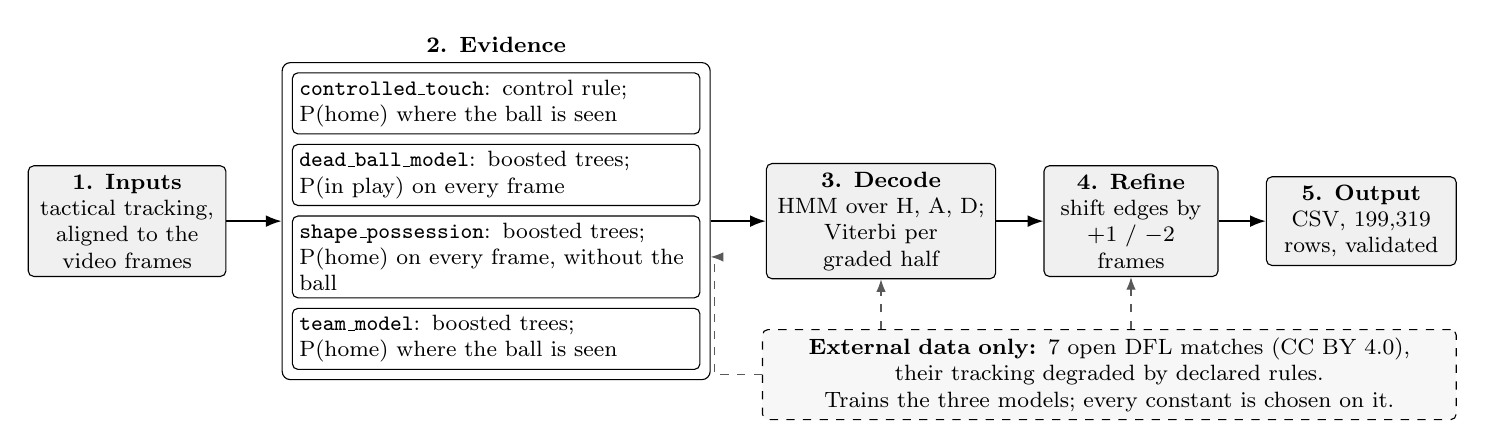
\begin{tikzpicture}[
  font=\footnotesize,
  stage/.style={draw, rounded corners=2pt, align=center, fill=black!6, minimum height=11mm, inner sep=3pt},
  src/.style={draw, rounded corners=2pt, align=left, fill=white, text width=50mm, inner sep=2.5pt},
  ext/.style={draw, dashed, rounded corners=2pt, align=center, fill=black!3, inner sep=3pt},
  flow/.style={-{Latex[length=2mm]}, semithick},
  learn/.style={-{Latex[length=1.6mm]}, dashed, black!65}]
% the four sources, stacked
\node[src] (s1) {\code{controlled\_touch}: control rule;\\ P(home) where the ball is seen};
\node[src, below=1.2mm of s1] (s2) {\code{dead\_ball\_model}: boosted trees;\\ P(in play) on every frame};
\node[src, below=1.2mm of s2] (s3) {\code{shape\_possession}: boosted trees;\\ P(home) on every frame, without the ball};
\node[src, below=1.2mm of s3] (s4) {\code{team\_model}: boosted trees;\\ P(home) where the ball is seen};
\node[draw, rounded corners=3pt, inner sep=3.5pt, fit=(s1)(s4),
      label={[font=\footnotesize\bfseries]above:2. Evidence}] (ev) {};
\node[stage, left=7mm of ev, text width=23mm] (in) {\textbf{1. Inputs}\\ tactical tracking, aligned to the
  video frames};
\node[stage, right=7mm of ev, text width=27mm] (de) {\textbf{3. Decode}\\ HMM over H, A, D;\\ Viterbi per
  graded half};
\node[stage, right=6mm of de, text width=20mm] (re) {\textbf{4. Refine}\\ shift edges by\\ $+1$ / $-2$ frames};
\node[stage, right=6mm of re, text width=22mm] (out) {\textbf{5. Output}\\ CSV, 199{,}319 rows, validated};
\draw[flow] (in) -- (ev);
\draw[flow] (ev) -- (de);
\draw[flow] (de) -- (re);
\draw[flow] (re) -- (out);
% external data
\node[ext, text width=86mm, anchor=north east] (dfl) at ($(out.south east)+(0,-8mm)$)
  {\textbf{External data only:} 7 open DFL matches (CC~BY~4.0),\\ their tracking degraded by declared rules.\\
   Trains the three models; every constant is chosen on it.};
\draw[learn] (dfl.west) -- ++(-6mm,0) |- (ev.east |- s3.east);
\draw[learn] (dfl.north -| de.south) -- (de.south);
\draw[learn] (dfl.north -| re.south) -- (re.south);
\end{tikzpicture}
\caption{The pipeline. Solid arrows carry the provided match through the five stages at run time. Dashed arrows
show where learned models and chosen constants come from: other games only, never the provided match.}
\label{fig:pipeline}
\end{figure*}

\subsection{The decoder}
A three-state hidden Markov model over \code{H}, \code{A} and \code{D} is decoded by Viterbi over each graded half.
Each source adds its log-likelihood to the states it speaks for; silence adds nothing. A change of team has a cost
(6 nats), a change into or out of \code{D} a larger one (32), and a run lasts at least 1.4\,s for a team and 1\,s
for \code{D}. A possession is then an interval whose two edges must be paid for, which is what spellF1 scores. A
last step moves a change of team 1 frame later and a change into \code{D} 2 frames earlier: the pipeline's own
median lag on the benchmark, negated.

\subsection{Why this and not something else}
The rules allow training and tuning on external data only. So the three models are trained on other matches, and
every numeric constant is chosen on a benchmark of other matches (Section~\ref{sec:validation}). Boosted trees on
hand-built features suit that: they train on a CPU, are committed as JSON files, and each feature can be checked
against how our tracking differs from the training data. The decoder is there because spellF1 punishes flicker:
evidence may be noisy per frame, but a possession has to be worth its two edges.

\section{Assets Used and Dropped}

Table~\ref{tab:assets} lists the provided assets.

\begin{table}[t]
\caption{The provided assets}
\label{tab:assets}
\centering
\footnotesize
\begin{tabularx}{\columnwidth}{@{}>{\raggedright\arraybackslash}p{22mm}>{\raggedright\arraybackslash}p{8mm}L@{}}
\toprule
Asset & Used & How, or why not \\
\midrule
Tactical tracking (ATD) & yes & The only input of every source. \\
Smart Tagging & no & Automatic tags; their confidence could only be measured on this match, which the rules
  forbid, so the source was removed before submission. \\
Tactical homography & no & Analysed only: the camera's aim is too coarse a proxy for the ball (median error 12\,m
  along the pitch). \\
Tactical video and audio & no & A whistle detector on the audio was tried and failed its gate. \\
Broadcast video, tracking, homography & no & Its own timeline with cuts and replays, and no mapping to the
  tactical frames. \\
Public 5-minute ground truth & check only & A correctness check of the finished pipeline
  (Sections~\ref{sec:data} and~\ref{sec:validation}). \\
\bottomrule
\end{tabularx}
\end{table}

\textbf{Tried and dropped,} each by a bar declared before its run (docs/results.md in the repository has the
numbers): the restarting team by restart type; the referee's whistle; the camera's aim as a ball proxy; repairing
wrong-team track slots; a pretrained event model (PathCRF~\cite{kim2026}); recalibrating the shape model per half;
placing edges by the decoder's posterior; the broadcast's ball inside our gaps; and several further features and
decoder variants in the last week. None of them is in the submitted configuration.

\section{Training Data}
\label{sec:data}

We labelled nothing by hand, on any game. Everything learned comes from one external dataset
(Table~\ref{tab:data}).

\begin{table}[t]
\caption{The labelled dataset behind every model and constant}
\label{tab:data}
\centering
\footnotesize
\begin{tabularx}{\columnwidth}{@{}p{19mm}L@{}}
\toprule
Data & DFL/IDSSE open data~\cite{bassek2025}: \code{BallStatus} (in play or dead) and \code{BallPossession} (the
  team), per frame \\
Source, licence & Bassek et al. 2025, figshare, CC BY 4.0 \\
Who labelled it & DFL, in its official match data; the paper says operators check all data \\
How much & 7 full matches (2 Bundesliga, 5 2.~Bundesliga), 25\,Hz, 668 graded minutes \\
Used for & Training the three models; choosing every constant; validation. Its 681 restart events only as a
  diagnostic of a dropped source \\
\bottomrule
\end{tabularx}
\end{table}

Three other external sources were read and nothing in the submission stands on them: PathCRF's public
checkpoint~\cite{kim2026} (MPL-2.0; measured once, dropped); SkillCorner's open data~\cite{skillcorner} (MIT; a
plausibility check of the benchmark's ball gaps, made after they were declared); and the events of Metrica's three
sample games~\cite{metrica} (used once to measure how fine possession is in our provider's data, then withdrawn on
5~Nov because the data has no licence; ranking on two truths, Section~\ref{sec:validation}, was kept on its own
ground: neither is known to be right).

\textbf{Nothing was trained, fitted or tuned on the provided game.} No tracking was corrected by hand, no
human-produced data about the match was used, and no output of ours was checked against the video. The public
5~minutes were used as a correctness check (alignment, a valid and deterministic file, each source pointing the
right way) and inspected to understand what counts as possession; no model saw them and no constant of the
submission was set on them.

\textbf{Three things we state openly:}
\begin{itemize}
\item \emph{Two published figures.} The benchmark's degradation (Section~\ref{sec:validation}) quotes two
  statistics of this match from the organisers' DATA.md: the ball is missing on 41\% of the graded frames, and
  20.5 objects are tracked on average. We read them as public information of the task statement, given to every
  team, not as use of the provided data.
\item \emph{An earlier benchmark, retired.} Until 9~Nov the degradation was fitted on label-free statistics of our
  own tracking (which frames have no ball, how long the tracklets are). After the organisers' reply of 5~Nov
  (``anything that is not explicitly allowed is not permitted'') we retired it, retrained the models and chose
  every constant again on a degradation that measures nothing of our match. Only the architecture (which
  components exist, the trees' settings) comes from the old one, re-verified on the new.
\item \emph{The Smart Tagging,} a source in earlier versions, was removed for the same reason
  (Table~\ref{tab:assets}).
\end{itemize}

\section{Missing and Noisy Tracking}

\begin{itemize}
\item \textbf{Long ball gaps.} No interpolation: gaps under 2\,s hold 0.1\% of the missing frames. The decoder
  keeps its state through a gap, and the shape model speaks inside it (out of fold on the benchmark, the
  submitted version names the right team on 86\% of the in-play frames without a ball).
\item \textbf{A missing ball is not a dead ball.} \code{D} never comes from ball presence alone; the dead-ball model
  reads where the ball vanished and reappeared and how the players behave.
\item \textbf{The ball-speed channel is unusable} (empty on 92\% of the frames with a ball). Every speed comes
  from successive positions.
\item \textbf{Track slots are tracklets, not players} (46 slots for 22 players). No feature follows a slot over
  time; the shape features are aggregates over each team's players.
\item \textbf{Wrong-team slots.} One team shows more than 11 slots on at least 10.8\% of the graded frames. Such
  slots do not cluster at the ball, so a repair was judged not worth it; this stays a limitation
  (Section~\ref{sec:limits}).
\end{itemize}

\section{Possession Rules Implemented}
\label{sec:rules}

\begin{itemize}
\item \textbf{Control.} A team controls the ball when the nearest tracked player is its own and within 1.5\,m, no
  opponent is within 1.0\,m, and the ball moves with that player (relative speed at most 6\,m/s): a proximity
  rule in the line of~\cite{link2017} and~\cite{vidal2022}. A run of such frames votes for its team from its
  first frame, so a change lands where control began.
\item \textbf{Loose balls} (a pass in flight, a rebound). While the ball is seen but nobody controls it, the rule
  keeps a weaker vote for the last controlling team. Possession stays with that team unless the other evidence
  outweighs it.
\item \textbf{Challenges.} With an opponent within 1\,m there is no control, so the previous team keeps the ball
  until one side controls it. A touch of a frame or two becomes a possession only if the evidence around it pays
  the decoder's switch cost and lasts 1.4\,s.
\item \textbf{Dead ball and restarts.} \code{D} is the dead-ball model's, and every graded frame before a half's
  documented kick-off is \code{D}. After a restart the weaker vote still favours the team that had the ball
  before the stoppage, until a player controls the ball; we do not use the restart type. Who owns a dead ball is
  not asked.
\item \textbf{A change of team inside a ball gap} falls where the shape evidence for the other team pays the
  switch cost.
\item \textbf{Not implemented:} aerial duels (no ball height), pass and interception events, and abstention (tried
  and dropped: no \code{X} on a graded frame).
\end{itemize}

\section{Validation and Results}
\label{sec:validation}

\subsection{The benchmark}
The public window holds 17 possessions and is the best-tracked part of the match, so it cannot rank anything, and
the rules forbid tuning on it. We validate on the seven DFL matches instead. The truth is built as ours is
(\code{D} where the ball is dead, else the team in possession), the tracking is degraded to resemble ours by rules
declared before any run (ball gaps of 1 to 60\,s covering 41\% of the frames, players dropping out, 46 slots), and
the official scorer grades each half. DFL's possession flag is fine-grained and the grain of ours is unknown, so
every choice is ranked on the mean of two truths: DFL's own (``raw'') and one that absorbs possessions under 5\,s
(``coarse''). Every change had to clear a bar declared before its run, tested over the seven matches.
Table~\ref{tab:results} has the scores.

\begin{table}[t]
\caption{Pooled spellF1 on the benchmark (seven matches, three seeds)}
\label{tab:results}
\centering
\footnotesize
\begin{tabularx}{\columnwidth}{@{}Lcc@{}}
\toprule
Configuration & Raw & Coarse \\
\midrule
Nearest player + majority vote, the organisers' baseline (the better of its 50- and 125-frame windows) & 0.1885 &
  0.2092 \\
Touch rule + dead-ball model + shape model + HMM & 0.5414 & 0.5829 \\
+ shape model version 2 and the team model: \textbf{the submission} & \textbf{0.5891} & \textbf{0.5963} \\
\bottomrule
\end{tabularx}
\end{table}

Measured before the last two models were added: on the mean of the two truths, the score falls by 0.10 without
the shape source and by 0.03 without the touch rule. A perfect dead-ball source would add only 0.03 to 0.04, a
perfect team source about 0.2 where the ball is seen and 0.10 to 0.18 inside the gaps: what is left to win is who has the ball.

\subsection{On our match, checks that pass or fail only}
The file validates, has no \code{X} on a graded frame and comes out byte-identical on repeated runs. Its \code{D}
share is 34.4\% of the graded frames, inside a band set on DFL; it holds 386 possessions (\code{H} 38.2\%,
\code{A} 27.4\%). On the public window it scores macroF1 0.7199 and spellF1 0.4737: a check for gross errors,
which chose nothing.

\section{Limitations}
\label{sec:limits}

\begin{itemize}
\item \textbf{A change of team inside a ball gap is found late; this is the largest error left.} On the
  benchmark, where the ball is seen a change lands within a few frames; inside a gap it lands late (a median of 6
  frames at a possession's start and 11 at its end, the upper quartile near one second). Late in each half the
  ball is missing on up to 80\% of a 5-minute block, and there the team rests on the shape model alone, trained on
  other teams.
\item \textbf{The benchmark is not our tracking.} Its ball gaps ignore the play, while ours fall where the tracker
  loses the ball (more often near the lines), and it has no wrong-team slots. So its scores are not a forecast
  for the real match; it overstates the dead-ball model in particular, by an amount we cannot measure.
\item \textbf{The team model has no transfer check on our match,} and wrong-team slots hit it hardest, since it
  reads distances per team. The benchmark's test of this realised a team with more slots than players on at most
  2.3\% of the graded frames; our match shows one on at least 10.8\%.
\item \textbf{Seven German matches,} five of them one club's home games: the models may transfer imperfectly to
  LaLiga, and several constants were chosen within noise of their neighbours.
\item \textbf{Our truth's conventions are unknown:} how short a possession may be, and when exactly \code{D}
  starts and ends. The models carry DFL's conventions, and the decoder's minimum of 1.4\,s, chosen on the
  benchmark, rules out shorter possessions, which the public truth shows to exist.
\end{itemize}

\textbf{With more time:} recover the ball from the video with a detector trained on other matches; place the
edges from detected passes; learn our provider's timing from other games of the same provider, given data with a
licence.

\section{Reproduction}

Unpack the data bundle into \code{data/} as \code{data/README.md} describes, then run from the repository root
(on macOS or Linux: \code{python3.11} and \code{.venv/bin/python}):

{\scriptsize
\begin{verbatim}
py -3.11 -m venv .venv
.venv/Scripts/python -m pip install -r requirements-pipeline.txt
.venv/Scripts/python pipeline/run.py pipeline/configs/main.toml
\end{verbatim}
}

\code{evaluation/results/main.csv} is the file the last command writes from \code{data/}. The run validates it
with the official checks and prints its sha256; the uploaded \code{Un Dia de Partit.csv} is that file renamed. Its sha256 is

{\scriptsize
\begin{verbatim}
aae79a0446dabdf565d86b95f03acf0a53b5698cf3d80033c25bf7d49cbd3bdb
\end{verbatim}
}

Python 3.11.9; every package the pipeline imports is pinned (numpy 2.4.6, pandas 3.0.6). The models are JSON files
in \code{pipeline/models/}, so nothing is trained at run time and no GPU is needed; the run takes under a minute
on a laptop CPU. On 16~Nov the file came out with the same sha256 from fresh clones of the public repository, in
fresh environments, on two processors: an AMD Ryzen~5 5500U laptop (Windows, Python 3.11.9) and an Apple M2
(macOS, Python 3.11.18). Earlier versions were also rebuilt under Linux. Retraining the models and repeating the benchmark needs only the public DFL files:
\code{requirements-benchmark.txt} and the commands in \code{pipeline/benchmark/README.md}. The full record of
every experiment, with its numbers, commands and failures, is in \code{docs/results.md}, and our reading of the
rules in \code{docs/rules.md}.

\begin{thebibliography}{6}
\bibitem{bassek2025} M. Bassek, R. Rein, H. Weber, and D. Memmert, ``An integrated dataset of spatiotemporal and
  event data in elite soccer,'' \emph{Scientific Data}, vol. 12, art. 195, 2025. Data: figshare,
  doi:10.6084/m9.figshare.28196177 (CC BY 4.0; we degrade its tracking).
\bibitem{kim2026} H. Kim \emph{et al.}, ``PathCRF: Ball-free soccer event detection via possession path inference
  from player trajectories,'' in \emph{Proc. KDD}, 2026, arXiv:2602.12080.
\bibitem{link2017} D. Link and M. Hoernig, ``Individual ball possession in soccer,'' \emph{PLOS ONE}, 2017.
\bibitem{vidal2022} F. Vidal-Codina \emph{et al.}, ``Automatic event detection in football using tracking data,''
  \emph{Sports Engineering}, 2022, arXiv:2202.00804.
\bibitem{skillcorner} SkillCorner, ``Open data: broadcast tracking of A-League matches,'' MIT licence.
\bibitem{metrica} Metrica Sports, ``Sample data,'' github.com/metrica-sports/sample-data.
\end{thebibliography}

\end{document}
